\subsection{FAST}
Um m�todo de reconhecimento baseado em detec��o de arestas originalmente desenvolvido por Edward Rosten
 e Tom Drummond no seu paper  Machine learning for high-speed corner
 detection in 2006 (Later revised it in 2010) A maior promessa do m�todo � a efici�ncia computacional
O m�todo considera um c�rculo de dezesseis pixels ao redor da aresta considerada p. 
O detector original [13],[14] classifica p como uma aresta se existem n pixels 
cont�guos em um c�rculo que s�o mais brilhantes do que o pixel candidato de intensidade Ip mais
 um threshold t ou mais escuros do que Ip-t

 \begin{figure}[h!]
\centering
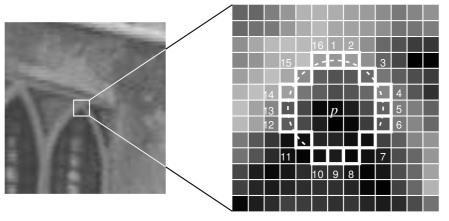
\includegraphics[scale=0.8]{images/fast01}
\caption{FAST}
\label{fig:fast01}
\end{figure}


Na imagem~\ref{fig:fast01} foi escolhido n=12. Um teste r�pido �
\begin{enumerate}
	\item  selecionar o ponto � testar primeiro as extremidades. no caso da imagem, escolhido o ponto p
	\item Compara-se os pontos 1 e 9, e verifica-se se o ponto p tem intensidade com diferen�a de m�dulo t, ou seja os pontos 1 e 9 s�o mais claros ou mais escuros do que o ponto p pelo fator de t
	\item Caso o ponto p continue sendo um candidato, avalia-se os pontos 5 e 13
	\item Se p � uma aresta ent�o pelo menos 3 desses pontos devem ser mais brilhantes ou mais escuros do que p ent�o o teste pode ser feito nos demais pontos.
\end{enumerate}

